This section regards material taught during class.

\subsection{Apache Wayang}

Apache Wayang (\cite{58d56a9c6f264d75800463fbb4117538}) is a framework that provides systematic solution to the problem of having to select and learn a specialized platform for data analytics. Wayang is a unified framework that can execute a data pipeline over any set of platforms seamlessly and efficiently.

There are four main issues with the current data analytics workflow that Apache Wayang aims to address. First is \textbf{Platform Independence}. There are currently many different data analytics platforms, all with different APIs, written in different languages, and with different strengths and weaknesses. A typical data analysis pipeline involves using several different platforms for different parts of the pipeline to ensure efficiency. This is a large burden for developers as it may require re-implementing pipelines in, and learning, new APIs and languages, as well as possibly requiring custom-made scripts for interfacing between these various platforms. Wayang solves these problems by being platform-agnostic, as well as capable of automatically determining what platform individual parts of the pipeline should run on, ensuring that the developer only needs to use a single framework.

This also extends into the second issue and solution, \textbf{Opportunistic Cross-Platform}. As mention above, it can be valuable to make use of several different platforms in the same pipeline to make use of the strengths and weaknesses of each platform. Since Wayang can automatically determine the best platform for a given task, it can always choose the best platform for each task in a pipeline, being cross-platform and efficient. Adjacent to this is also the problem of being \textbf{Mandatory Cross-Platform}. Even if efficiency is irrelevant for the data analysis pipeline, it may still be necessary to use multiple platforms, as different data analytics platforms have different sets of features. If a pipeline requires two functions, each of which are exclusive to two different platforms, then the pipeline will be forces to make use of both. Wayang's dynamic platform selection trivialises this.

Finally is the issue of \textbf{Polystore}, that is, having data in various different data stores. Normally, this would have the developer write different preprocessing scripts for importing the various data formats, but Wayang can dynamically import data from various data lakes, without a developer having to specify how.

A fifth boon not mentioned in the original paper is \textbf{Migration}. As an organization expands their architecture, Apache Wayang expand their platform support, or as platforms get deprecated or obsolete, code written for Apache Wayang can be easily migrated to these new platforms by simply changing which plugins are being used. This allows pipeline migrations that would normally require significant investment to be done very easily, thus future-proofing Apache Wayang pipelines for as long as Wayang is actively maintained.

\subsection{Request log analysis}

This section involves extracting the total number of distinct IP addresses that have connected to each domain in a log file from a web server. The log is formatted as follows:

\begin{small}
\begin{verbatim}
66.24.69.97 -- [17/May/2024:10:25:44 +0000] "GET http://www.google.com/bot.html"
66.24.69.97 -- [17/May/2024:10:26:44 +0000] "GET https://itu.dk/research.html"
66.24.69.97 -- [17/May/2024:10:28:44 +0000] "GET https://itu.dk/programmes/bds.html"
71.19.157.179 -- [17/May/2024:10:30:12 +0000] "GET http://www.google.com/faq.html"
66.24.69.97 -- [17/May/2024:31:10:44 +0000] "GET https://itu.dk/contact.html"
\end{verbatim}
\end{small}

This can be achieved in 3 simple steps. The first step is extracting the IP addresses and the domains. This can be done using a simple regular expression. I have created a function that takes a line from the log as an input, and produces a key-value pair of the matched domain to the matched IP address:

\begin{minted}{python}
>>> def findMatches(s: str):
...     x_IP = "(?<IP>(?:\d{1,3}\.){3}\d{1,3})"
...     x_DOMAIN = "(?<DOMAIN>https?:\/\/(?:www)?[^\/]*\.[a-zA-Z]{2,3})"
...     match = re.search(f"{x_IP}.*{x_DOMAIN}", s)
...     return (match.group("DOMAIN"), match.group("IP"))
\end{minted}

This function can then be used in the PySpark \texttt{map} method after reading the file. This produces an RDD of the above mentioned key-value pairs. Since one IP address can visit the same domain multiple times, the distinct domain-IP pairs need to be extracted. This can be done using the \texttt{distinct} method which also works for tuples. Finally, the number of occurrences of each key can now be counted using the \texttt{countByKey} method, finally giving us the desired output.

\begin{minted}{python}
>>> sc.textFile("hdfs://log.txt")\
...     .map(findMatches)\
...     .distinct()\
...     .countByKey().items()
[("http://www.google.com", 2), ("https://itu.dk", 1)]
\end{minted}

Assuming that the underlying Spark platform has 3 available workers, a few steps will be made under the hood to answer this query. First, in the example above, the data is loaded from HDFS, or the Hadoop Distributed File System. This means that the 3 workers can load their part of the data individually, without having to wait for the driver to send their respective data. The subsequent \texttt{map} can be done each worker independently of the others. The \texttt{distinct} method however, relies on a call to \texttt{reduceByKey} under the hood. \texttt{reduceByKey} is an action that required aggregating the data from each worker to calculate the result. \texttt{countByKey} is similar. Since the results of both \texttt{distinct} and \texttt{countByKey} rely on information from all workers to ensure that no duplicates are present and all keys are counted respectively, they cannot be entirely run in an isolated manner, and network communication is necessary. See Figure \ref{fig:spark_execution} for a visualization of the query.

\begin{figure}
    \centering
    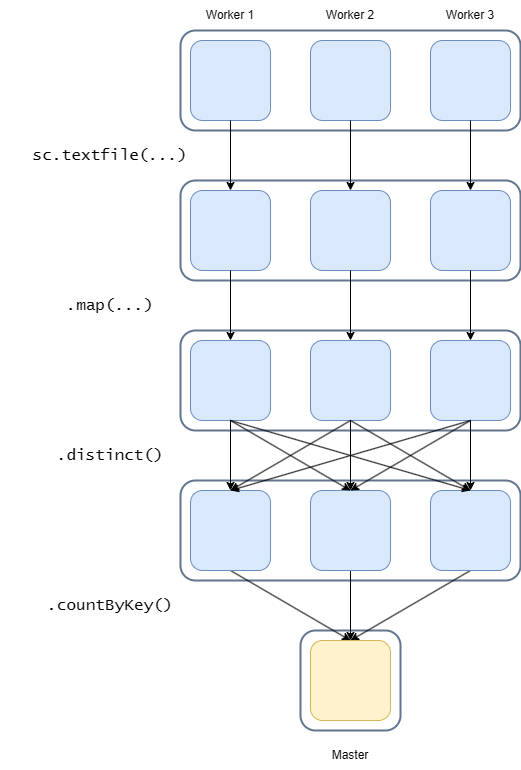
\includegraphics[width=0.3\linewidth]{images/death.drawio.png}
    \caption{Execution of simple spark query}
    \label{fig:spark_execution}
\end{figure}

\subsection{Principal Component Analysis}

Principal Component Analysis, or PCA, is a dimensionality reduction method. It works by calculating the vector along which the dataset has the largest variance. This vector is known as a Principal Component. It then repeats this process for as many principal components as there are dimension in the dataset, ensuring that each vector is orthogonal to all the previous ones. PCA is a very popular way to do dimensionality reduction because of it's ease of use and the fact that it preserves most of the variance in a dataset. 

PCA has however come under criticism for several shortcomings, chief among them being lack of efficiency on large dataset and difficulty of interpretability. To help address these issues, different variants of the original PCA have been made, primarily Incremental PCA to address performance issues, and Sparse PCA to address interpretability issues.

The efficiency issues of PCA stem from the need to perform computations on the entire dataset at once, requiring that the dataset is loaded into memory. This is impossible for larger datasets, as it is not uncommon to find datasets of several gigabytes or larger, especially in areas such as gene research. Incremental PCA addresses this by performing the computations in batches. This allows the algorithm to only load a small fraction of the total dataset into memory at any given time, updating its PCA estimation as it iterates through the dataset.

Interpretability is a problem for PCA, as every datapoint that results from a transformation by PCA becomes a linear combination of the original input variables. This makes it very hard to reason about individual datapoints after a PCA transformation, as every datapoint is dependent on every other datapoint to some extent. Sparse PCA attempts to address this by using a sparse set of input variables. That is, instead of using the entire input dataset for the linear combinations, it uses just a few input variables. This means that every transformed datapoint will only be a linear combination of a few input variables, which makes it much easier to reason about. 

\begin{figure}
    \centering
    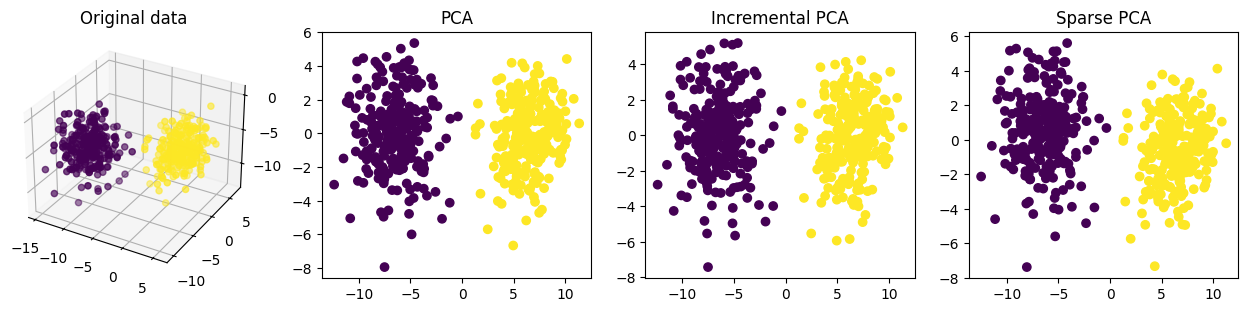
\includegraphics[width=1\linewidth]{images/pca.png}
    \caption{Original, randomly generated 3-dimensional dataset (left), as well as the same dataset reduced to 2 dimensions with PCA, Incremental PCA and Sparse PCA.}
    \label{fig:pca}
\end{figure}

Comparisons between the three variations of PCA can be seen in Figure \ref{fig:pca}. The plots are very similar, which shows that despite their added limitations, the PCA variations still match the performance of the original PCA very closely. It is important to note, however, that the dataset provided is already very linearly separable, which likely results in all the PCA variations very easily finding the optimal separability.

\subsection{Distributed and Federated Learning}

Traditionally, machine learning training tasks have been performed in a manner known as Distributed Learning. Here, a central server is responsible for training a model either by itself, or by using a distributed network of machines. This requires training data to be stored in a location accessible to each compute node involved in training the model. Data used for these tasks are usually publically accessible datasets, such as webscraping.

This can be an issue as a large amount of the data generated in the world is kept locally on individual devices such as smartphones and laptops. These data are also usually very sensitive, such as photos or text input, and are therefore difficult to collect in a secure and private manner. To address these problems and make use of the vast amount of sensitive on-device data, Federated Learning was created as an alternative to Distributed Learning. Where Distributed Learning has one or a particular set of machines serve as compute nodes for training a single central model, Federated Learning has each device contribute its own training data to optimize a local version of the global model, before then communicating weight updates to a centralized control server (\cite{DBLP:journals/corr/McMahanMRA16}). This allows Federated Learning to be used in cases where privacy is a big concern, such as the photos and text input from personal computing devices mentioned above, or applications such as medical patient data.